\documentclass{standalone}
\usepackage{tikz} % or other graphics packages you need
\usetikzlibrary{arrows.meta}

\begin{document}
\newcommand{\mysize}{\large}

% =========================================================================
% 1. DEFINE GLOBAL MODULE CONSTANTS (Accessible by all subroutines)
% =========================================================================
\newcommand{\gLmda}{0.1}
\newcommand{\gEps}{0.05}

% Universal dimensions for the structural outer boundary box
\pgfmathsetmacro{\xleft}{-1 - \gLmda}
\pgfmathsetmacro{\xright}{1 + \gLmda}
\pgfmathsetmacro{\ybottom}{0 - \gEps}
\pgfmathsetmacro{\ytop}{0.4}

% Colors
\colorlet{mygreen}{green!60!black}
\colorlet{myred}{red!80!black}

% Subroutine B: Draws the internal shaded distribution boxes
\newcommand{\drawShadedBoxes}[3]{% mu, sigma, color
    % Right variance block
    \shadedraw[left color=#3!70, right color=#3!10, draw=#3!0, very thin ] (#1,0) rectangle (#1 + #2, \ytop - \gEps);
    % Left variance block
    \shadedraw[left color=#3!10, right color=#3!70, draw=#3!0, very thin ] (#1,0) rectangle (#1 - #2, \ytop - \gEps);
}

% Subroutine C: Draws the grid elements, axis lines, and labels
\newcommand{\drawAxisGrid}{%
    % Horizontal baseline axis
    \draw[very thick] (\xleft,0) -- (\xright,0); 
    
    % Vertical reference ticks spanning from bottom margin up to the shade height
    \draw[ thick ] (-1, \ytop - \gEps) -- (-1, -\gEps);
    \draw[ thick ] (0, \ytop - \gEps)  -- (0, -\gEps);
    \draw[ thick ] (1, \ytop - \gEps)  -- (1, -\gEps);
}

% Subroutine D: Draws the indicator arrow locating the mean
\newcommand{\drawMeanArrow}[1]{% mu
    \draw[ very thick, black, -Stealth ] (#1, \ytop - \gEps) -- (#1,-0.0125);
}

\newcommand{\drawXlabels}{
    % Reference coordinate text labels
    \node[ below ] at (-1,-\gEps) {\mysize{Low}};
    \node[ below ] at (0,-\gEps) {\mysize{Moderate}};
    \node[ below ] at (1,-\gEps) {\mysize{Strong}};
}

% =========================================================================
% 3. ASSEMBLY GRAPHIC CONTAINER
% =========================================================================
\newcommand{\drawComponentGroup}[3]{% <--- FIXED: Added [3] to process arguments properly
    \drawShadedBoxes{#1}{#2}{#3}%    <--- Passes Group arg 1, 2, and 3 down to shaded boxes
    \drawAxisGrid%
    \drawMeanArrow{#1}%              <--- Passes Group arg 1 (mu) down to the arrow macro
}
% =========================================================================
%   Render image
% =========================================================================
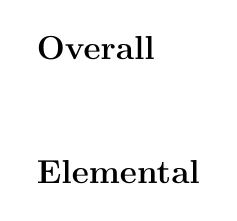
\begin{tikzpicture}[ scale = 3.5 ]

    % --- BOTTOM COMPONENT BLOCK ---
    % mu = 0.23, sigma = 0.43, Color = Green
    \begin{scope}[ yshift = 0cm ]
        \drawComponentGroup{0.23}{0.43}{mygreen}
   	    \drawXlabels
        % Label added to the right side of the axis line
        \node[anchor=west, font=\bfseries\large, xshift=0.15cm] at (\xright, 0.2) {Elemental};
    \end{scope}

    % --- TOP COMPONENT BLOCK ---
    % Shifted vertically up by exactly 0.45 units
    % mu = -0.15, sigma = 0.30, Color = Red
    \begin{scope}[ yshift = 0.45cm ]
        \drawComponentGroup{-0.15}{0.30}{myred}
        % Label added to the right side of the axis line
        \node[anchor=west, font=\bfseries\large, xshift=0.15cm] at (\xright, 0.2) {Overall};
    \end{scope}

\end{tikzpicture}

\end{document}
